\chapter{Contexte du stage}
\section{L'entreprise : Aboard Engineering}
Aboard Engineering est un bureau d'études en automatique, électronique et
informatique industrielle. Composé d'experts en contrôle et instrumentation de
systèmes embarqués temps réel, ses ingénieurs développent des solutions pour des
applications civiles et militaires. De la R\&D à la série, Aboard Engineering
travaille dans le domaine des transports (automobile, aéronautique, marin), de
l'off-road (agriculture, engins de chantier, ...) et de l'industrie. Les figures
\ref{fig:domaines} et  \ref{fig:metiers} sont tirées du site web d'Aboard
Engineering et récapitulent les domaines et métiers de la société.

\begin{figure}[h]
	\center
	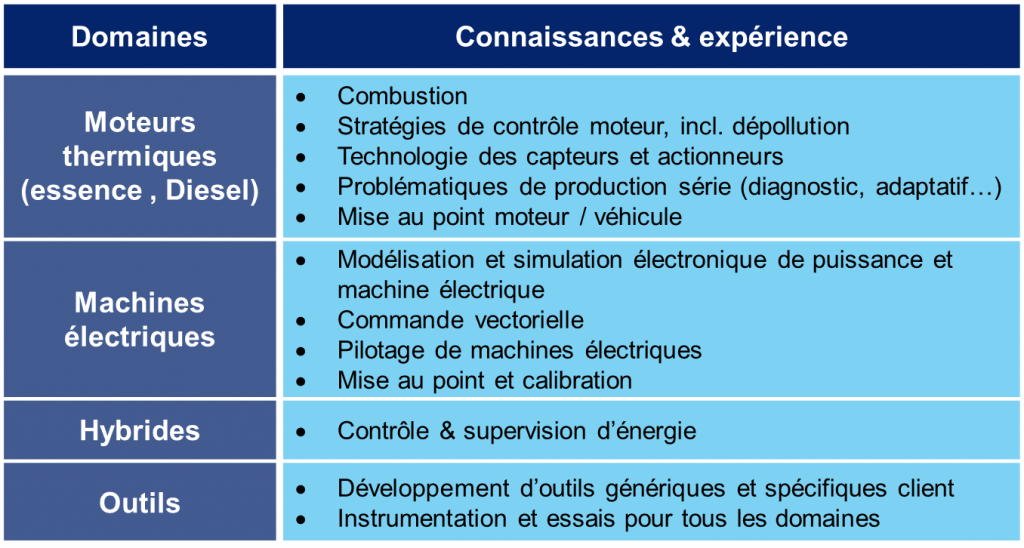
\includegraphics[scale=0.4]{images/domaines}
	\caption{Domaines -- Source : Abord Engineering}
	\label{fig:domaines}
\end{figure}

\begin{figure}[h]
	\center
	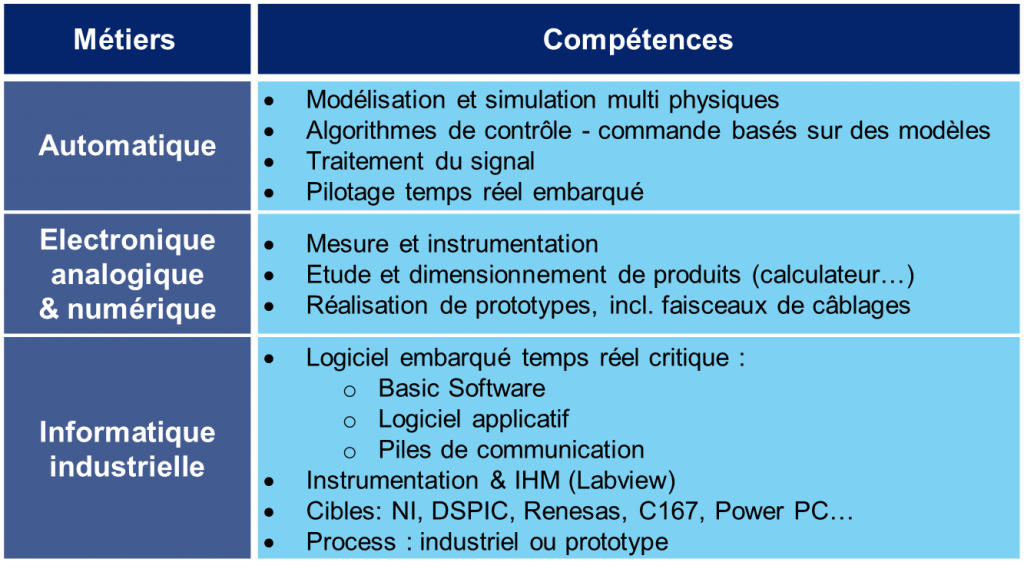
\includegraphics[scale=0.4]{images/metiers}
	\caption{Métiers et Compétences -- Source : Abord Engineering}
	\label{fig:metiers}
\end{figure}

\section{La plate-forme Orianne}
\label{sec:orianne}

Aboard Engineering fournie différents types de produits et de services. Je ne vais ici développer que le cas de la plate-forme \gloss{orianne} sur laquelle j'ai travaillé.

Orianne est une plate-forme de prototypage rapide de fonctions de contrôle moteur.
Elle permet de regrouper différents modules d'un calculateur moteurs (transmission, ABS, injection, couple moteur, etc.) afin de générer une unique application qui sera déployée dans un calculateur moteur.
Pour cela, une interface graphique permet de choisir quelles fonctions sont à intégrer dans l'application et de les configurer  mais aussi les caractéristiques du moteur cible ou la configuration du \gloss{rtos} (définition des récurrences des tâches).
Une fois l'application configurée, la plate-forme va chercher les codes sources des modules sélectionnés, génère les fichiers sources non fonctionnels (non relatifs à des fonctions moteurs) et effectue la compilation.
La sortie produite est un fichier binaire représentant le code source compilé ainsi qu'un fichier \og dictionnaire \fg{} associant chaque élément à l'adresse à laquelle il sera stocké dans la mémoire du calculateur. Ce fichier contient les adresses des constantes, des calibrations, des différentes fonctions appelées, etc.
L'intérêt d'avoir des adresses fixes et connues pour ces éléments est qu'il est possible via un logiciel tiers de récupérer ces informations et de les modifier directement dans la mémoire sans avoir à déployer une nouvelle application. Pour rappel, nous sommes dans un cadre R\&D et beaucoup de tests sont effectués sur banc de tests et le besoin d'adapter les calibrations pour obtenir le meilleur comportement est primordial.

La plate-forme en elle-même est composée de plusieurs outils :
\begin{itemize}
	\item Configuration du moteur cible
	\item Configuration des fonctions moteur
	\item Configuration du RTOS
	\item Génération des fichiers sources non fonctionnels
	\item Compilation de l'application
\end{itemize}

\section{L'environnement de travail}
J'avais mon poste de travail personnel sur lequel j'avais un contrôle suffisant pour installer les logiciels qu'il me fallait.
L'entreprise possède également plusieurs ordinateurs portables sur lesquels sont installés certains logiciels comme Matlab\up{\circledR}, \gloss{inca} ou \gloss{canalyzer}. Ces ordinateurs portables sont en libre service aux employés pour l'utilisation des ces logiciels en particuliers ou simplement pour avoir un environnement de test indépendant de l'environnement de développement.

J'ai utilisé les logiciels suivant durant mon stage :
\begin{description}
  \item[Netbeans/Eclipse/IntelliJ] J'ai utilisé plusieurs IDE. Les deux premiers pour reprendre le code existant et comprendre l'architecture des projets. Le dernier par préférence personnelle et par habitude.
  \item[VirtualBox] J'ai installé deux machines virtuelles sur mon poste de travail en utilisant le logiciel VirtualBox. La première sous Fedora pour faire de l'analyse statique de code C. La deuxième sous Debian configurée en serveur pour installer Gitlab.
  \item[Gitlab] J'ai mis en place un Gitlab pour gérer mes sources. Gitlab est une plate-forme de gestion de projet permettant d'héberger un dépôt Git et de gérer des tâches (similaire au service Github mais sur un serveur local).
\end{description}

